
\chapter{A szimuláció eredményei}

Mostanra láttuk azt, hogy milyen modellekkel dolgozunk és azt is, hogy ezt szépen össze lehet gyúrni egy alkalmazásba. Azt viszont még nem láttuk, hogy ezek konkrétan milyen eredményeket is produkálnak. Az alábbiakban több szempontból is megvizsgáltuk azt, hogy a \cite{archetti2016cooperation} cikkbeli modell, illetve annak általunk kiegészített változata, hogyan viselkedik.

Kezdetben a szimuláció pontosságának megvizsgálása érdekében a már rendelkezésünkre álló bemeneti paraméterekre (melyeket Archetti is használt \cite{archetti2016cooperation}) elvégeztünk 100-100 szimulációt, minden egyes diffúziós távolságra 1-től 5-ig.

A bemeneti paraméterek az alábbiak voltak:
\begin{itemize}
	\item populáció mérete: 1000
	\item defektálók: 5\%
	\item generációk száma: 15
	\item kooperálók költsége: 0.01
	\item osztódás: nincs
\end{itemize}

A \eqref{eq:payoffGradient} és \eqref{eq:diffGradient} függvények paraméterei, melyeket az elkövetkezendő szimulációk során használtunk:
\begin{itemize}
	\item $s = 2$
	\item $k = 1$
	\item $d = \frac{1}{2}D$
	\item $z = 20$
\end{itemize}

\begin{figure}[ht!]
	\centering
	\begin{tabular}{cc}
		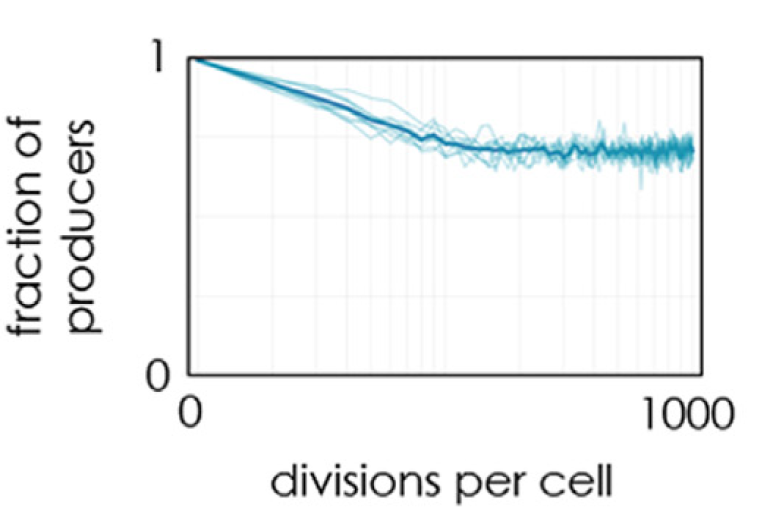
\includegraphics[width=0.47\linewidth]{images/arc_dist2}
		&
		\includegraphics[width=0.47\linewidth]{images/dist2}
		\\
		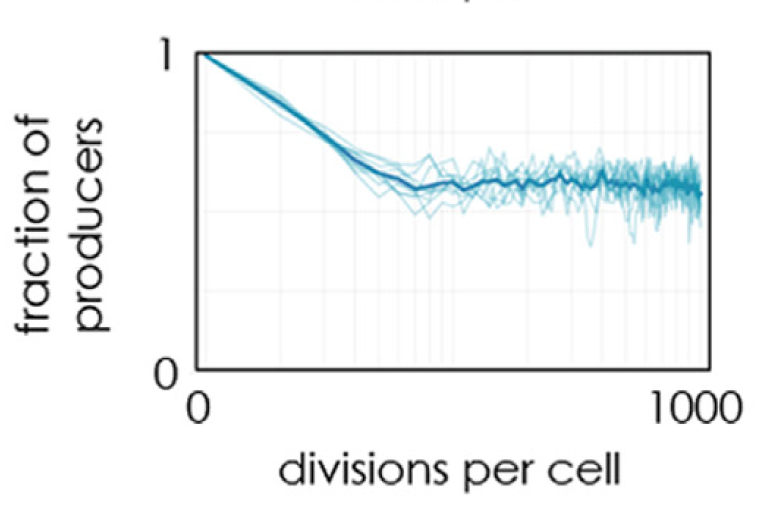
\includegraphics[width=0.47\linewidth]{images/arc_dist3}
		&
		\includegraphics[width=0.47\linewidth]{images/dist3}
		\\
		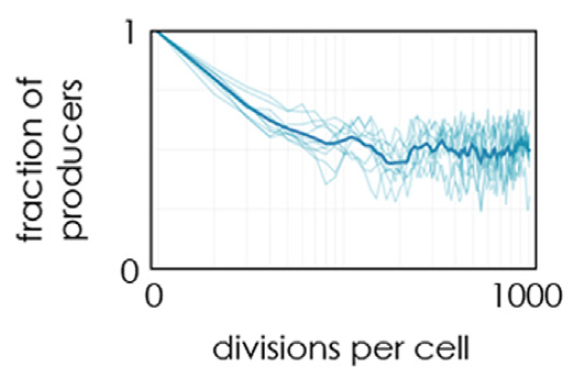
\includegraphics[width=0.47\linewidth]{images/arc_dist4}
		&
		\includegraphics[width=0.47\linewidth]{images/dist4}
		\\
		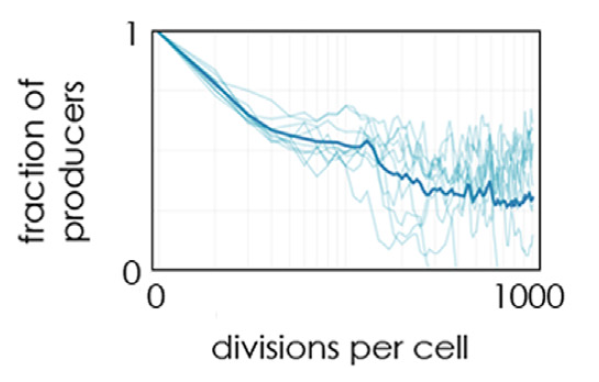
\includegraphics[width=0.47\linewidth]{images/arc_dist5}
		&
		\includegraphics[width=0.47\linewidth]{images/dist5}
		\\
	\end{tabular}
	\caption{Szimulációs eredmények a fenti paraméterekre. Bal oldalt az \cite{archetti2016cooperation} cikkbeli grafikonok, míg jobb oldalt az általunk generált grafikonok. Látható, hogy mi is hasonló eredményeket kaptunk.}
	\label{fig:DistChange}
\end{figure}

Megállapítottuk, hogy ugyanarra az eredményre (Ábra \ref{fig:DistChange}) jutottunk mi is mint Archetti (\cite{archetti2016cooperation}), a fenti paraméterekre a kooperálók aránya hasonlóan viselkedik, igaz kisebb eltérések ugyan mutatkoztak. Míg mi minden esetben 100 szimulálást végeztünk, addig ő csak 10-et, így a kis eltéréseket ennek tulajdoníthatjuk.

Ezzel projektünk első mérföldkövét leraktuk, megbizonyosodtunk arról, hogy az általunk implementált modell visszaadja az eredetit. Most már kísérletezhetünk különböző paraméterekkel, hogy megvizsgáljuk a populáció viselkedését. Egy pár esetet a következő fejezetekben tárgyalunk.

\section{A költség és nyereség hatása}

Mint ahogyan azt már láttuk, a kooperáló sejtek termelési költsége nagyban befolyásolja a játék végkimenetelét (Ábra \ref{fig:CoopCostChange}), ami nem nagy meglepetés, hisz minél többe kerül a termelés annál jobban megéri élősködni. Az esetek többségében a defektálás a legkifizetődőbb, de alacsony költségek mellett fenntartható egy bizonyos egyensúly is a két fél között, sőt, extrém körülmények (paraméterek) mellett az is elérhető, hogy a teljes populáció a kooperálás mellett döntsön. 

\begin{figure}[ht!]
	\centering
	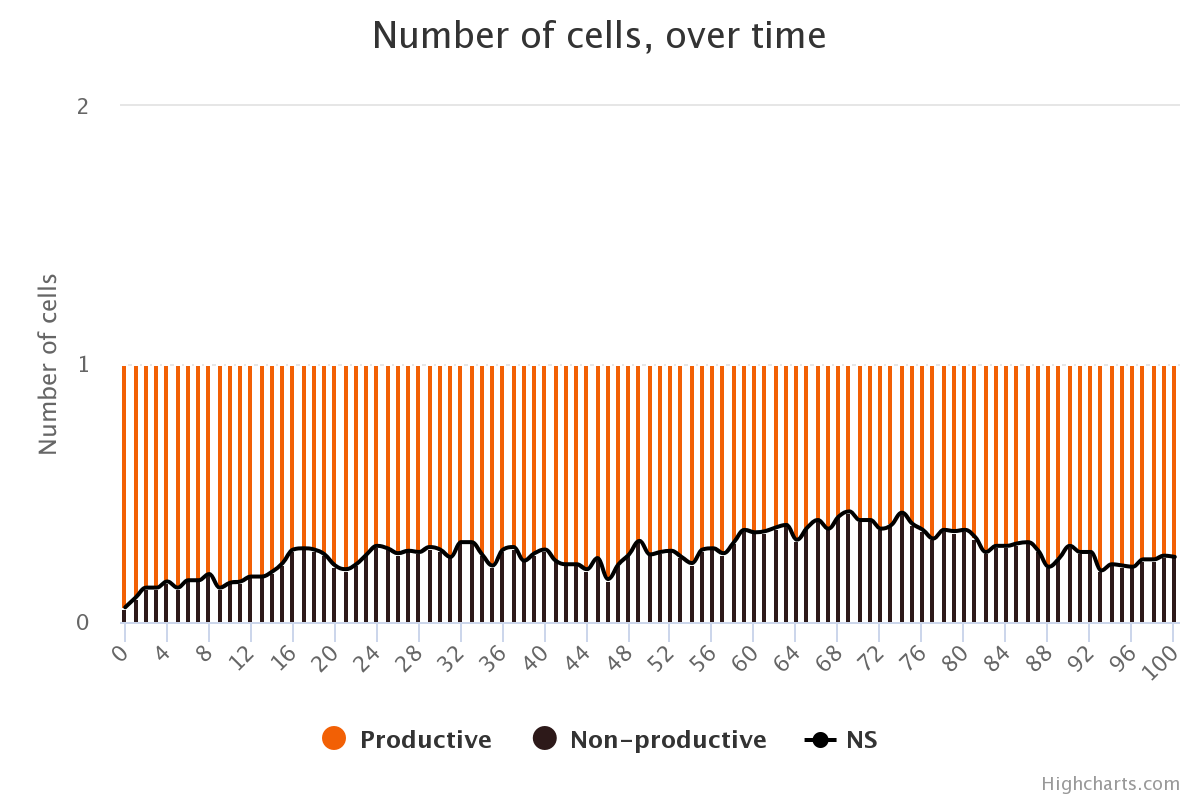
\includegraphics[width=0.9\linewidth]{images/egyensuly}
	\captionsetup{justification=centering}
	\caption{Egyensúlyi helyzet alakulása 100 generáción át amikor a költség 0.05 és a kezdeti defektálók aránya 5\%}
	\label{fig:egyensuly}
\end{figure}

Ha $cost \in\interval{0.01}{0.1}$ intervallumnak, akkor az eseteke döntő többségében egyensúlyi helyzethez jutunk (Ábra \ref{fig:egyensuly}). Azért csak a döntő többségében, mert, a játékszabályoknak köszönhetően, a véletlen is elég nagy szerepet játszik a játék alakulásában és nagyon ritkán történhet olyan, hogy az egyik stratégia dominál.

\begin{figure}[ht!]
	\centering
	\begin{tabular}{ccc}
		\includegraphics[width=0.32\linewidth]{images/chart001.jpeg}
		&
		\includegraphics[width=0.32\linewidth]{images/chart01.jpeg}
		&
		\includegraphics[width=0.32\linewidth]{images/chart08.jpeg}
	\end{tabular}
	\caption{A játék végkimenetele mikor a költségek rendre 0.01, 0.1 és 0.8}
	\label{fig:CoopCostChange}
\end{figure}


\section{Diffúziós távolság hatása}

Mint ahogyan azt már említettük, nem csak az elsőfokú szomszédokat vehetjük figyelembe, hanem egy bizonyos diffúziós távolságon belül található összes sejtet. Úgy néz ki, hogy ez a legkényesebb paraméterünk amelyet változtatni lehet. Ezen érték növelésével a valósághoz közelibb eredményeket kaphatunk. Sajnos nem állnak rendelkezésünkre erre vonatkozó adatok a biológiából, így csak egy pár, már más által is használt értékekre végeztünk kísérleteket és néztük meg, hogy milyen hatást vált ki ezen érték változása (Ábra \ref{fig:DiffDist}). 

\begin{figure}[ht!]
	\centering
	\captionsetup{justification=centering}
	\begin{tabular}{cc}
		\includegraphics[width=0.47\linewidth]{images/diffdist2}
		&
		\includegraphics[width=0.47\linewidth]{images/diffdist5}
	\end{tabular}
	\caption{A játék végkimenetele két diffúziós távolságra. A paraméterek: 160 sejt, 5\% defektáló, 0.3 költség, távolság: 2 illetve 5}
	\label{fig:DiffDist}
\end{figure}

Megfigyelhető, hogy a távolság növekedésével a defektáló sejtek jóval könnyebben terjednek el, nem csak a közvetlen szomszédokat befolyásolják, hanem a tőlük távolabb elhelyezkedőeket is. Meg kell jegyeznünk, hogy ezt a paramétert a hasnyálmirigyrák esetén megállapították (\cite{archetti2015heterogeneity}), valamint az is biztos, hogy az esetek túlnyomó részében ez az érték 5-10-től 30-60-ig terjedhet (\cite{archetti2016cooperation}).

\section{Osztódásra képes populációk}

Eddigi szimulációink során a populáció mérete állandó volt, és egy adott modellt követett. A már említett Gompertz-modellt (\ref{eq:gompertz}) beépítve a modellbe és az alkalmazásba (a felhasználói webes felületen csak egy checkbox, azaz akar-e a felhasználó osztódást) újabb szimulációkat futtattunk. Az \ref{fig:Divide} ábra szemlélteti azt az esetet amikor a sejtek osztódni is képesek és nem csak stratégiát váltani. 

\begin{figure}[ht!]
	\centering
	\begin{tabular}{cc}
		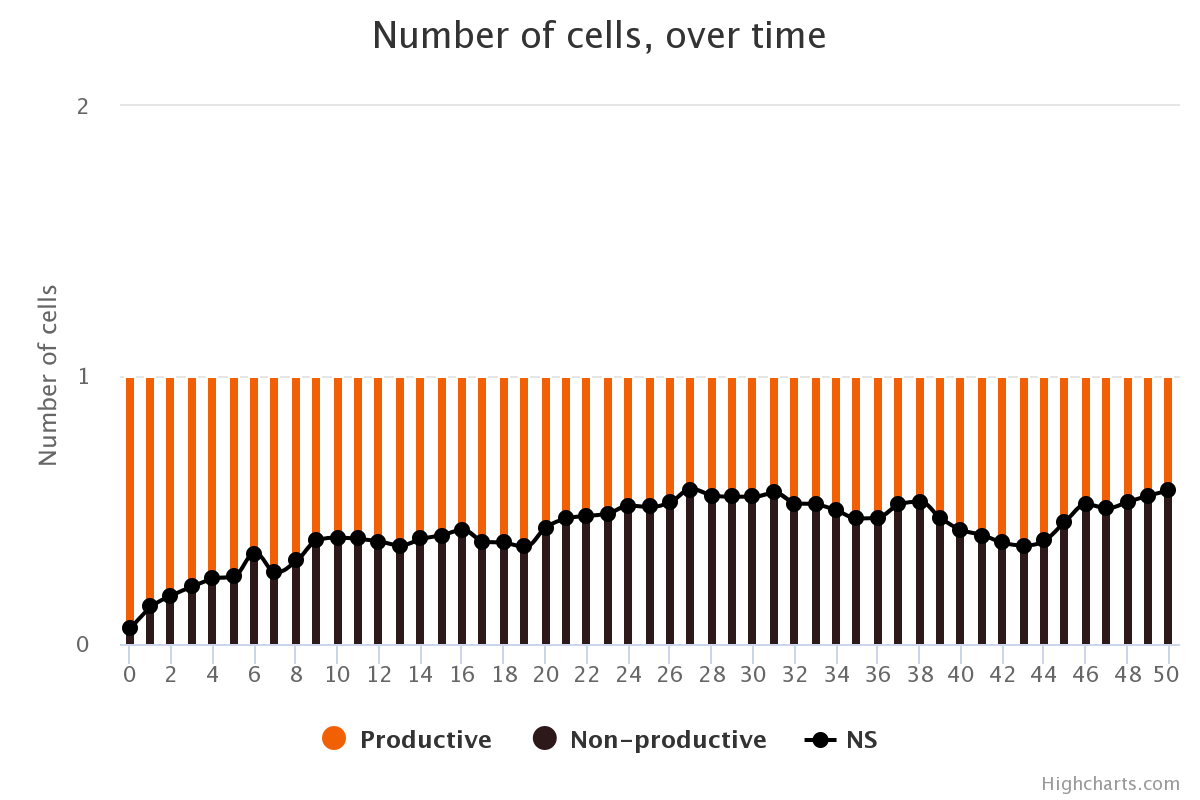
\includegraphics[width=0.47\linewidth]{images/nemosztodik}
		&
		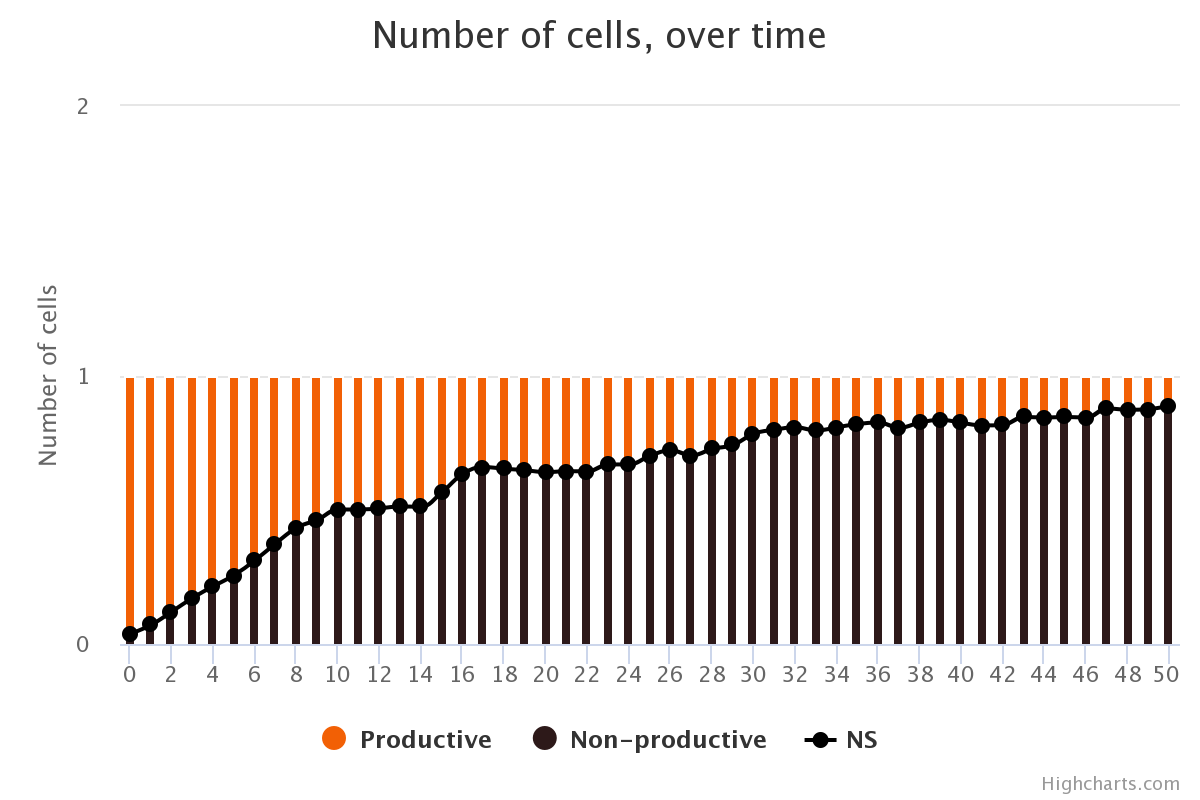
\includegraphics[width=0.47\linewidth]{images/osztodik}
	\end{tabular}
	\captionsetup{justification=centering}
	\caption{Az első esetben a sejtek nem osztódtak míg a másodikban igen, ugyanazon paramétereket felhasználva}
	\label{fig:Divide}
\end{figure}


Ez eddigiekben a sejtek csak átvehették a szomszéd stratégiáját, ami bizonyos szinten tekinthető osztódásnak. Feltételezve azt, hogy az a sejt amelyik átveszi a szomszéd stratégiáját elhal és az ő helyére kerül az osztódás utáni párja a szomszédnak, akkor egy fajta osztódást kapunk. Viszont a valóságban a sejtek nem csak területileg szaporodnak el, hanem számosságban is nőnek. Ezért éreztük szükségességet az osztódás bevezetésének.

Megfigyelhető, hogy az osztódás során létrejött új sejtek képesek felgyorsítani a defektálók terjedését, sőt, ahogyan az az \ref{fig:Divide} ábrán is látszik, míg az első esetben beáll az egyensúlyi helyzet, addig a második esetben még egyensúlyra utaló jeleket sem találunk. Ezen területen még további kísérletek szükségesek, hogy pontosabb képet kapjunk arról, hogy ez mennyire befolyásolja a játék végkimenetelét valamint ez mennyiben javít, esetleg ront, a modell valósághűségén.

Az is megvizsgáltuk, hogy átlagban mennyire tér el a két modell egymástól, ezért az eddig használt paraméterekkel legeneráltunk egy újabb populációt, mely már osztódásra is képes (\ref{table:osztodik} táblázat). Ezen eredményeket összevetettük azon modellel ahol nem volt osztódás (\ref{table:nemOsztodik} táblázat). Látható, hogy a kooperálók aránya (CoopPerc) kisebb amikor a sejtek osztódnak, de a szórása is nő.

\begin{table}[htb]
	\centering
	\begin{tabular}{ | l | l | l | l | l | l | l | l | l | l | l | l | }
		\hline
		\multirow{3}{*}{D = 2}
		& Generáció & 1 & 2 & 3 & 4 & 5 & 6 & 7 & 8 & 9 & 10 \\ \cline{2-12}
		& CoopPerc & 0.91 & 0.91 & 0.85 & 0.81 & 0.77 & 0.75 & 0.73 & 0.71 & 0.69 & 0.68 \\ \cline{2-12}
		& stdev & 0.01 & 0.01 & 0.02 & 0.03 & 0.03 & 0.03 & 0.05 & 0.05 & 0.05 & 0.06 \\ \hline
		\multirow{3}{*}{D = 3}
		& Generáció & 1 & 2 & 3 & 4 & 5 & 6 & 7 & 8 & 9 & 10 \\ \cline{2-12}
		& CoopPerc & 0.9 & 0.9 & 0.83 & 0.77 & 0.72 & 0.68 & 0.66 & 0.64 & 0.62 & 0.6 \\ \cline{2-12}
		& stdev & 0.02 & 0.02 & 0.03 & 0.04 & 0.04 & 0.05 & 0.04 & 0.05 & 0.05 & 0.04 \\ \hline
	\end{tabular}
	\vspace*{1mm}
	\caption{Osztódás nélküli modell}
	\label{table:nemOsztodik}
\end{table}

\begin{table}[htb]
	\centering
	\begin{tabular}{ | l | l | l | l | l | l | l | l | l | l | l | l | }
		\hline
		\multirow{3}{*}{D = 2}
		& Generáció & 1 & 2 & 3 & 4 & 5 & 6 & 7 & 8 & 9 & 10 \\ \cline{2-12}
		& CoopPerc & 0.87 & 0.87 & 0.79 & 0.74 & 0.7 & 0.67 & 0.64 & 0.61 & 0.59 & 0.57 \\ \cline{2-12}
		& stdev & 0.02 & 0.02 & 0.03 & 0.04 & 0.05 & 0.06 & 0.07 & 0.05 & 0.07 & 0.07 \\ \hline
		\multirow{3}{*}{D = 3}
		& Generáció & 1 & 2 & 3 & 4 & 5 & 6 & 7 & 8 & 9 & 10 \\ \cline{2-12}
		& CoopPerc & 0.89 & 0.9 & 0.82 & 0.75 & 0.7 & 0.66 & 0.62 & 0.59 & 0.56 & 0.54 \\ \cline{2-12}
		& stdev & 0.03 & 0.04 & 0.05 & 0.06 & 0.08 & 0.08 & 0.08 & 0.09 & 0.09 & 0.09 \\ \hline
	\end{tabular}
	\vspace*{1mm}
	\caption{Osztódást használó modell}
	\label{table:osztodik}
\end{table}
